\section{Experiments}
\label{sec:feats_results}
This chapter starts by giving visual results of our superpixel segmentation. We then elaborate on the experimental setup. The results from training and evaluation procedures are described. Details on method-specific parameters and configuration are also given.

\subsection{Superpixel Segmentation}
\label{sec:superpix}
Fig. \ref{fig:sp_example} shows examples of the superpixel segmentation.

\begin{figure}[htbp]
  \centering
  \includegraphics[width=11cm]{prev_sps}
  \caption[Superpixel segmentation example]{Example of superpixel segmentation on each type of sequence. Generated with \cite{achanta12}, with $200$ segments.
  Superpixel contours are in white, ground truth annotation is in red, and user-provided 2D location is in green}
  \label{fig:sp_example}
\end{figure}

Table \ref{tab:sp_errors} shows for each sequence type the maximum F1 score one would obtain while working with SLIC superpixels in a segmentation setup.

Intuitively, this measure increases as the number of superpixels increase.
We use here $N=1200$ superpixels, and note that increasing this value further does not improve the F1-score.

\begin{table}[htbp]
\centering
\caption{Superpixelization errors}
\label{tab:sp_errors}
\begin{tabular}{lp{1.8cm}}
\toprule
{} &               F1 \\
Types    &                  \\
\midrule
Brain    &  $0.92 \pm 0.02$ \\
Cochlea  &  $0.92 \pm 0.01$ \\
Slitlamp &  $0.92 \pm 0.02$ \\
Tweezer  &  $0.95 \pm 0.01$ \\
\bottomrule
\end{tabular}
\end{table}


\subsection{Neural Network Training}
In this section, we first describe the training configurations followed by the parameterization of the data augmentation.
We then analyze the training loss (learning curves) on few examples.
Visual examples of activation maps are given to illustrate what kind of filters the network is learning.

\subsubsection{Training Configurations} \label{ch:training_conf}
All of our U-Net based models are trained using the Adam optimizer \cite{kingma15} (learning rate $= 0.0001$, $\beta_1 = 0.9$, $\beta_2 = 0.999$, $\epsilon = 10^{-8}$, no decay).
Weights are initialized with the Glorot method \cite{glorot10}.
The stopping criterion for training is reached after $20$ epochs.

The maximum size of the mini-batch depends on the GPU memory, the model architecture, and since the latter has different input sizes, also the resolution of the input data.
We trained our models on a \textit{GeForce GTX 1080 Ti}, with 11GB memory.
The model architectures are all similar in size except for the \textit{U-Net Gaze Prob LSTM}, which contains another recurrent part.
The datasets also have similar resolution except for the \textit{CT Inner Ear A + B}.
Tab. \ref{tab:batch_size} shows the used mini-batch size.
\vspace{30pt}

\begin{table}[htbp]
   \centering
   \caption[Mini-batch size]{Mini-batch size used for training U-Net based methods. All methods are trained on a \textit{GeForce GTX 1080 Ti} GPU. Since the CT datasets are smaller in resolution, we could take larger mini-batches. The \textit{U-Net Gaze Prob LSTM} has a larger model and uses, therefore, smaller mini-batches.}
   \begin{tabular}{|c||c|c|}
      \hline
      \diagbox{Dataset}{Method} & \textbf{U-Net Gaze Prob LSTM} & \textbf{All others} \\
      \hline
      \hline
      \Gape[2pt][2pt]{\textbf{\makecell[c]{CT Inner Ear\\ A + B}}} & 4 & 16 \\
      \hline
      \Gape[11pt][11pt]{\textbf{All others}} & 1 & 4 \\
      \hline
   \end{tabular}
   \label{tab:batch_size}
\end{table}

\clearpage
\subsubsection{Data Augmentation} \label{results_data_gen}

The data augmentation parameters are given in Tab. \ref{tab:data_gen_param}.
Example frames are shown in \ref{fig:data_gen}.

\begin{table}[!htbp]
   \centering
   \caption[Data generator parameters]{Parameters of data generator. Rotation, translation, and shearing are used as transformation. Gaussian noise is also added to augment data variance. It is defined by the standard deviation $\sigma$, which is relative to the range in bit depth $0-255$. $2'000$ images are randomly sampled for each epoch.}
   \begin{tabular}{l|c}
      \toprule
      \textbf{Parameter} & \textbf{Value} \\
      \midrule
      Rotation range & $\pm11.25$° \\
      Horizontal translation range & $20\%$ of image width \\
      Vertical translation range & $20\%$ of image height \\
      Shearing range & $\pm22.5$° \\
      \midrule
      Gaussian noise $\sigma$ & $13$ \\
      \midrule
      Number of samples per epoch & $2'000$ \\
      \bottomrule
   \end{tabular}
   \label{tab:data_gen_param}
\end{table}
\vspace{30pt}

\begin{figure}[!htbp]
  \centering
  \includegraphics[width=\textwidth]{unet/data_gen}
  \caption[Examples of data generator]{Examples of data generator on an image of dataset \textit{Slit-Lamp Retina A}. We used rotation, translation, shearing and added Gaussian noise to each of the channels. The values are shown in Tab. \ref{tab:data_gen_param}.}
  \label{fig:data_gen}
\end{figure}

% ch\clearpage
% \subsubsection{Learning Curve} \label{ch:learning_curve}
% In our setting, we train the CNN model on the dataset we later extract the features from.
% Thus, there is no need to split the dataset into training and validation.
% The performance would even become worse since the model would be trained on fewer data.
% For our datasets, where all frames within the set are very similar to each other, we do not expect to find any signs of overfitting given the learning curve.

% However, since we will later describe an experiment that shows the feature performance versus the training time of the model (chapter \ref{ch:perf_vs_training}), we still investigate the training curve.
% To do so, we took the \textit{CT Inner Ear A} dataset and randomly split it into $80\%$ training set and $20\%$ validation set.
% Subsequently, we trained two models, namely a \textit{U-Net Rec} with MSE-loss and a \textit{U-Net Gaze Prob} with BCE-loss, for $500$ epochs.
% After each trained epoch, we calculated training and validation loss.
% Fig. \ref{fig:learn_curve} shows the training and validation loss for the given models.
% As we expected, there is no sign of overfitting.
% We also performed this experiment on other datasets and they all showed similar behaviour.
% \vspace{20pt}

% \begin{figure}[!htbp]
%   \centering
%   \subfloat[Learning curve of model \textit{U-Net Rec} on dataset \textit{CT Inner Ear A}]
%   {
%     \includegraphics[width=11cm]{learning_curve/learning_curve_ds11_rec}
%   }
%   \\
%   \subfloat[Learning curve of model \textit{U-Net Gaze Prob} on dataset \textit{CT Inner Ear A}]
%   {
%     \includegraphics[width=11cm]{learning_curve/learning_curve_ds11_prob}
%   }
%   \caption[Model learning curves]{Learning curves of training (a) \textit{U-Net Rec} and (b) \textit{U-Net Gaze Prob} model on dataset \textit{CT Inner Ear A}. We split the dataset into $80\%$ training and $20\%$ test and calculated the given loss after each trained epoch. As expected, there are no signs of overfitting.}
%   \label{fig:learn_curve}
% \end{figure}
% \vspace{20pt}

% The time per epoch largely depends on the input size of the model. If using the data generator with the above-mentioned settings and train the model on the stated hardware, it takes at most $4.5$ minutes per epoch (dataset \textit{Surgical Video Sequence}) and at least $35$ seconds per epoch (dataset \textit{CT Inner Ear A}).

\clearpage
\subsubsection{Activation Maps} \label{ch:act_maps}
To visualize the effect of filters (kernels) in a CNN, one often visualizes their activation during a forward pass.
The examples that follow correspond to the layer where our features are extracted, i.e. the last ReLU of the deepest layer (chapter \ref{feat_extract}). We randomly picked an image, performed a forward pass on a trained \textit{U-Net Rec} model, and visualized $11$ out of the $512$ activation maps. Fig. \ref{fig:activatiom_maps} shows two examples on dataset \textit{MRI Brain A} (Fig. \ref{fig:subfig:activatiom_map_ds09}) and \textit{Slit-Lamp Retina B} (Fig. \ref{fig:subfig:activatiom_map_ds13}). The upper left image shows the input image, and the other plots the activation maps, respectively.

We observe for both examples activation maps that have excitations at the object of interest's location. Thus, the filters are able to capture the foreground region. The fact that no activation maps are fully black indicate that their associated filters effectively contribute to the feature vector. Due to zero-padding used in the convolutional layers, border-effect occur. We will discuss this effect later in chapter \ref{ch:zero_vs_sym_pad}.
\vspace{30pt}

\begin{figure}[!htbp]
  \centering
  \subfloat[Example on \textit{MRI Brain A}]
  {
    \label{fig:subfig:activatiom_map_ds09}
    \includegraphics[height=6.2cm]{activation_maps/activations_ds09_0097}
  }
  \hfill
  \subfloat[Example on \textit{Slit-Lamp Retina B}]
  {
    \label{fig:subfig:activatiom_map_ds13}
    \includegraphics[height=6.2cm]{activation_maps/activations_ds13_0109}
  }
  \caption[Activation maps]{Activation maps of a trained \textit{U-Net Rec} model. The upper left image shows the passed image from (a) \textit{MRI Brain A}, and (b) \textit{Slit-Lamp Retina B} datasets. The other $11$ plots show some randomly chosen activation maps, extracted at the deepest level after the last ReLU.}
  \label{fig:activatiom_maps}
\end{figure}

\clearpage
\subsection{Feature Extracting Methods}
We provide results of the evaluation of our feature extraction methods. The evaluation procedure's configurations are first described. Second, the numerical values of the parameters of our methods are given. Third, we show the influence of using data augmentation. Fourth, we give experimental results on the feature performance vs. training-time. Fifth, the influence of the selected features of Random Forest is observed. Sixth, we present an overall ranking of the feature extraction methods in terms of \textit{max F1-Score}. Lastly, we investigate the influence of zero-padding.

\subsubsection{Configurations of Evaluation Procedure} \label{ch:eval_configs}
In chapter \ref{optimization} we stated that weight initialization of neural networks can be crucial for performance. Depending on the initialization, the gradient-based optimization will end in different minima and thus, might not be very constant. One could seed the random number generators, such that it always produces the same output. Anyhow, since we compare between different methods, seeding the random number generators would not allow a fair comparison.

U-Net based methods are evaluated in ten repetitions, i.e. each model is trained ten times on each dataset, resulting in ten different feature sets per dataset and method. We evaluate each feature matrix individually by the Random Forest classifier. Its settings are described in chapter \ref{random_forest}. For evaluation, the Random Forest is not seeded.

Concerning the baseline methods (including \textit{VGG-16}), the overall performance is largely unaffected by the random initialization. Thus, for those methods, we produced only one feature matrix per method and dataset. However, the Random Forest, in turn, is applied ten times on each feature matrix.

\subsubsection{Parameterization of Feature Extraction Methods}
We now give the numerical values of the parameters of our models. The parameters of the baseline methods are given first, followed by the U-Net based method's parameters. For detailed information on the methods, refer to chapter \ref{ch:methods}.

\subsubsection{Baseline Methods}
Tab. \ref{tab:baseline_params} shows the different parameters used for all baseline methods. For comparison purpose, both \textit{ScSP} and \textit{BoVW}, have $512$ classes and a SIFT keypoint size of $16 \times 16$ pixels. The number of keypoints used for vector quantization is defined in terms of number per image for the \textit{BoVW} method, and number over the entire sequence for the \textit{ScSP} method. We experimented with the patch size used for the \textit{ScSP} and \textit{VGG-16} methods. For \textit{ScSP}, taking the width as three times the average width of superpixels ($MSPW$) leads to best results. For the \textit{VGG-16} method, the optimal patch size is found to be two times the $MSPW$. We define:

\begin{equation}
   MSPW = \frac{1}{S} \sum_{i=1}^S \sqrt{A_i}
   \label{eq:mspw} 
\end{equation}
\vspace{6pt}

Where $S$ is the number of superpixels in the sequence and $A \in \mathbb{Z}$ the area of the individual superpixel measured in pixels. 

\clearpage
\begin{table}[!htbp]
   \centering
   \caption[Baseline parameters]{Illustration of parameters used in the baseline methods. The individual methods are described in chapter \ref{ch:baselines}.}
   \begin{tabular}{c|m{1.3cm}|c|l}
      \toprule
      \textbf{Method} & \textbf{Symbol} & \textbf{\makecell{Feature \\ Dimension $D$}} & \textbf{Parameters}\\
      \midrule
      BoVW & \makecell{\includegraphics[width=1cm]{icons/bovw}} & $512$ & 
        \makecell[l]{Number of classes = $512$ \\ 
                  SIFT KP size = $16 \times 16$px \\
                  Number of KP for CB per image = $100$} \\
      \midrule
      ScSP & \makecell{\includegraphics[width=1cm]{icons/scsp}} & $10'752$ & 
        \makecell[l]{Number of classes = $512$ \\ 
                  SIFT KP size = $16 \times 16$px \\
                  Number of KP for CB over all sequence = $20'000$ \\
                  Pyramid levels = $[1,2,4]$ \\
                  Patch width and height = $3 \cdot MSPW$} \\
      \midrule
      VGG-16 & \makecell{\includegraphics[width=1cm]{icons/vgg}} & $4'096$ & 
        \makecell[l]{Patch width and height = $2 \cdot MSPW$} \\
      \bottomrule
      \multicolumn{4}{c}{KP $\coloneqq$ keypoint \hspace{14pt} CB $\coloneqq$ codebook \hspace{14pt} MSPW $\coloneqq$ mean superpixel width} \\
      \bottomrule
   \end{tabular}
   \label{tab:baseline_params}
\end{table}
\vspace{20pt}

\subsubsection{U-Net Based Methods}
Tab. \ref{tab:unet_params} give the values of the parameters of our U-Net based models. For methods that predict a probability map $\boldsymbol{\hat{Z}}$, we set $\sigma$ to $6\%$ of the image width. For methods that involve the probability map $\bm{Z}$ in their loss-functions, we set $\sigma$ to $30\%$ of the image width. Fig. \ref{fig:prob_maps} shows ($\boldsymbol{Z}/\max{\{\boldsymbol{Z}\}}$) with the two $\sigma$ values mentioned above.
\vspace{30pt}

\begin{table}[!htbp]
   \centering
   \caption[U-Net based method parameters]{Illustration of parameters used in the U-Net based methods.}
   \begin{tabular}{l|m{3.3cm}|l}
      \toprule
      \textbf{Method} & \textbf{\makecell{Symbol}} & \textbf{Parameters}\\
      \midrule
      U-Net Gaze Rec & \makecell{\includegraphics[width=1cm]{icons/unet_gaze_rec}} & 
        \makecell[l]{$\sigma = 30\%$ of image width} \\
      \midrule
        \makecell[l]{U-Net Gaze Prob \\
                     U-Net Gaze Prob Freeze \\
                     U-Net Gaze Prob Concat} & 
      \makecell{\includegraphics[width=1cm]{icons/unet_gaze_prob} \includegraphics[width=1cm]{icons/unet_gaze_prob_freeze} \includegraphics[width=1cm]{icons/unet_gaze_prob_concat}} & 
        \makecell[l]{$\sigma = 6\%$ of image width} \\
      \midrule
      U-Net Gaze Prob LSTM & \makecell{\includegraphics[width=1cm]{icons/unet_gaze_prob_lstm}} & 
        \makecell[l]{$\sigma = 6\%$ of image width \\
                     $\alpha = 0.2$} \\  
      \bottomrule
   \end{tabular}
   \label{tab:unet_params}
\end{table}

\clearpage
\begin{figure}[!htbp]
  \centering
  \subfloat[$\sigma = 6\%$ of image width]
  {
    \includegraphics[width=6cm]{probability_maps/prob_map_06}
  }
  \hfill
  \subfloat[$\sigma = 30\%$ of image width]
  {
    \includegraphics[width=6cm]{probability_maps/prob_map_30}
  }
  \caption[Illustration of probability maps]{Visualization of probability map ($\boldsymbol{Z}/\max{\{\boldsymbol{Z}\}}$). In (a), we show the probability map for methods that predict $\boldsymbol{\hat{Z}}$. (b) shows the probability map of method \textit{U-Net Gaze Rec}.}
  \label{fig:prob_maps}  
\end{figure}

\subsection{Importance of Data Augmentation} \label{ch:nec_data_gen}
To explore the importance of data augmentation, we trained a \textit{U-Net Rec} model once with standard configuration (use of data generator) and once without using the data generator. As for all experiments, we performed the training and evaluation with ten repetitions, then took the mean \textit{max F1-Score}. We performed this experiment on one dataset per image modality. The results are summarized in Tab. \ref{tab:data_gen_nec}.
\vspace{30pt}

\begin{table}[!htbp]
   \centering
   \caption[Importance of data generator]{Influence of data augmentation in terms of mean \textit{max F1-Score} over ten repetitions. A \textit{U-Net Rec} model is trained in standard configuration, i.e. using data agumentation and without using data augmentation.}
   \begin{tabular}{l|*{4}{c|}}
      \toprule
       & \rotatebox[origin=cB]{90}{\parbox[t]{3.2cm}{\hspace{3pt} \textbf{Surgical Video} \hspace*{\fill}}} 
       & \rotatebox[origin=cB]{90}{\parbox[t]{3.2cm}{\hspace{3pt} \textbf{MRI Brain A} \hspace*{\fill}}} 
       & \rotatebox[origin=cB]{90}{\parbox[t]{3.2cm}{\hspace{3pt} \textbf{CT Inner Ear A} \hspace*{\fill}}} 
       & \rotatebox[origin=cB]{90}{\parbox[t]{3.2cm}{\hspace{3pt} \textbf{Slit-Lamp A} \hspace*{\fill}}} \\
      \midrule
      Data Augmentation \textbf{not in use} & 0.9826 & 0.9792 & 0.9587 & 0.9800 \\\midrule
      Data Augmentation \textbf{in use} & 0.9832 & 0.9810 & 0.9621 & 0.9863 \\\midrule\midrule
      \textbf{Gain} by using Data Augmentation & \textbf{0.061\%} & \textbf{0.184\%} & \textbf{0.355\%} & \textbf{0.643\%} \\
      \bottomrule
   \end{tabular}
   \label{tab:data_gen_nec}
\end{table}

\clearpage
\subsection{Performance w.r.t Training Time} \label{sec:perf_vs_training}
We now evaluate the performance of our features with respect to training time.
We trained a \textit{U-Net AE} model for $100$ epochs and run our evaluation pipeline every $10$ epochs.
Similar to all of our evaluations, we did the training and evaluation with ten repetitions to reduce variance.
Fig. \ref{fig:perf_vs_training} shows the mean \textit{max F1-Score} for one dataset per image modality.
We notice that past $20$ epochs the performance stagnates or even decreases for \textit{Cochlea A} dataset.
The next section provides more insight on that particular behaviour.
\vspace{30pt}

\begin{figure}[!htbp]
  \centering
  {
    \includegraphics[width=\textwidth]{f1_score_vs_training_time/f1_vs_training_rec}
  }
  \caption[Feature quality vs training time of U-Net Rec model]{Mean \textit{max F1-Score} over ten repetitions w.r.t training time using features from \textit{U-Net AE} for one dataset per image modality.}
  \label{fig:perf_vs_training}
\end{figure}

\clearpage
\subsection{Influence on Random Forest Feature Selection} \label{sec:infl_feat_selection}
Fig. \ref{fig:perf_vs_training_maxfeat} shows a comparison of performances for dataset \textit{Cochlea A} w.r.t parameter $m$, the number of sampled features of the Random Forest (see Sec. \ref{random_forest}).
We observe that setting $m=\sqrt{p}$, as advised by \cite[Ch. 15]{hastie09}, gives higher \textit{max F1-Scores} compared to $m=p$.
Both curves show a decreasing tendency.
\vspace{10pt}

\begin{figure}[!htbp]
  \centering
  {
    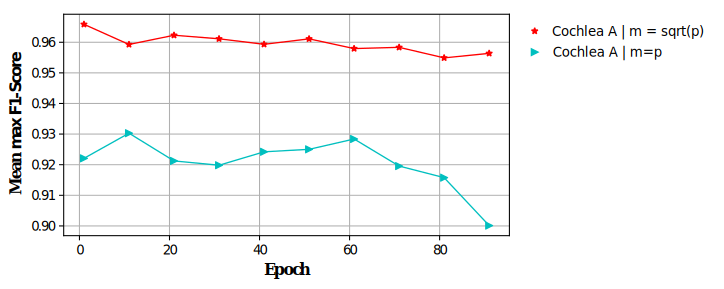
\includegraphics[width=\textwidth]{f1_score_vs_training_time/f1_vs_training_rec_maxfeat}
  }
  \caption[Feature quality vs training time of U-Net Rec model]{Mean \textit{max F1-Score} over ten repetitions w.r.t training time. The graph shows the results of \textit{U-Net Rec} model for dataset \textit{CT Inner Ear A}. The red curve illustrates the result when Random Forest selects $m=\sqrt{p}$ features and the cyan curve when selecting $m=p$.}
  \label{fig:perf_vs_training_maxfeat}
\end{figure}

Based on this observations, we choose to train our U-Net based models for $20$ epochs and set $m=\sqrt{p}$ in the following experiments.
\vspace{20pt}

\subsection{Method Comparison}
Tab. \ref{tab:final_results} summarizes the feature performance for each dataset and method in terms of \textit{max F1-Scores} averaged over ten repetitions.
All best scores per dataset are marked in red font.
For each dataset and method, we performed a two-sided Welch's t-test \cite{welch1947} to determine whether the score reached by the individual method is significantly different to the score reached by the best method for that dataset.
All values marked in bold font are not significantly different to the best score for a significance level of $0.05$.
The last row shows how many times the given method did not significantly perform worse than the best method.
We name this score \textit{Top-Sig-Score}.

\begin{table}[!htbp]
   \centering
   \caption[Feature quality]{Performance in terms of \textit{max F1-Scores} averaged over ten repetitions for each dataset and method, respectively. The according standard deviation is given underneath each score. Best scores per dataset are marked in red font. All bold marked scores are not significantly different from the best score when testing by a two-sided Welch's t-test with a significance level of 0.05. The last row shows on how many datasets the specific method was not significantly different to the best method.}
   \begin{tabular}{l|*{9}{c|}}
      \toprule
       & \rotatebox[origin=cB]{90}{\parbox[t]{4cm}{BoVW \hspace*{\fill}}} 
       & \rotatebox[origin=cB]{90}{\parbox[t]{4cm}{ScSP \hspace*{\fill}}} 
       & \rotatebox[origin=cB]{90}{\parbox[t]{4cm}{VGG \hspace*{\fill}}} 
       & \rotatebox[origin=cB]{90}{\parbox[t]{4cm}{U-Net AE \hspace*{\fill}}}
       & \rotatebox[origin=cB]{90}{\parbox[t]{4cm}{U-Net Prior AE \hspace*{\fill}}}
       & \rotatebox[origin=cB]{90}{\parbox[t]{4cm}{U-Net Pred Loc \hspace*{\fill}}}
       & \rotatebox[origin=cB]{90}{\parbox[t]{4cm}{U-Net Pred Loc Frozen \hspace*{\fill}}}
       & \rotatebox[origin=cB]{90}{\parbox[t]{4cm}{U-Net Motion Pred \hspace*{\fill}}}
       & \rotatebox[origin=cB]{90}{\parbox[t]{4cm}{U-Net Motion Pred LSTM \hspace*{\fill}}}  \\
       & \raisebox{-\totalheight}{\includegraphics[width=0.8cm]{icons/bovw}} 
       & \raisebox{-\totalheight}{\includegraphics[width=0.8cm]{icons/scsp}} 
       & \raisebox{-\totalheight}{\includegraphics[width=0.8cm]{icons/vgg}} 
       & \raisebox{-\totalheight}{\includegraphics[width=0.8cm]{icons/unet_rec}} 
       & \raisebox{-\totalheight}{\includegraphics[width=0.8cm]{icons/unet_gaze_rec}} 
       & \raisebox{-\totalheight}{\includegraphics[width=0.8cm]{icons/unet_gaze_prob}} 
       & \raisebox{-\totalheight}{\includegraphics[width=0.8cm]{icons/unet_gaze_prob_freeze}} 
       & \raisebox{-\totalheight}{\includegraphics[width=0.8cm]{icons/unet_gaze_prob_concat}} 
       & \raisebox{-\totalheight}{\includegraphics[width=0.8cm]{icons/unet_gaze_prob_lstm}}\\
      \midrule\midrule
      {\scriptsize Surgical Video} & \scriptsize 0.6649 & \scriptsize 0.8998 & \scriptsize 0.9647 & \textbf{\scriptsize 0.9830} & {\color{red} \textbf{\scriptsize 0.9832}} & \scriptsize 0.9791 & \scriptsize 0.9811 & \scriptsize 0.9776 & \scriptsize 0.9807 \\[-4pt]
       & \tiny $\pm$6.24e-4 & \tiny $\pm$6.04e-4 & \tiny $\pm$3.87e-4 & \tiny $\pm$4.84e-4 & \tiny $\pm$4.22e-4 & \tiny $\pm$1.84e-3 & \tiny $\pm$4.78e-4 & \tiny $\pm$2.93e-3 & \tiny $\pm$7.21e-4 \\\midrule\midrule
      {\scriptsize MRI Brain A} & \scriptsize 0.3163 & \scriptsize 0.9288 & \scriptsize 0.9666 & \textbf{\scriptsize 0.9774} & {\color{red} \textbf{\scriptsize 0.9810}} & \scriptsize 0.9764 & \textbf{\scriptsize 0.9806} & \scriptsize 0.9673 & \textbf{\scriptsize 0.9794} \\[-4pt]
       & \tiny $\pm$3.61e-3 & \tiny $\pm$5.05e-3 & \tiny $\pm$2.10e-3 & \tiny $\pm$4.65e-3 & \tiny $\pm$3.95e-3 & \tiny $\pm$3.30e-3 & \tiny $\pm$3.28e-3 & \tiny $\pm$8.90e-3 & \tiny $\pm$5.02e-3 \\\midrule
      {\scriptsize MRI Brain B} & \scriptsize 0.7502 & \scriptsize 0.8568 & \scriptsize 0.8911 & \textbf{\scriptsize 0.9232} & \textbf{\scriptsize 0.9292} & \scriptsize 0.9142 & \textbf{\scriptsize 0.9253} & {\color{red} \textbf{\scriptsize 0.9297}} & \scriptsize 0.9201 \\[-4pt]
       & \tiny $\pm$8.20e-3 & \tiny $\pm$7.36e-3 & \tiny $\pm$3.88e-3 & \tiny $\pm$5.63e-3 & \tiny $\pm$3.74e-3 & \tiny $\pm$8.59e-3 & \tiny $\pm$4.83e-3 & \tiny $\pm$7.09e-3 & \tiny $\pm$7.90e-3 \\\midrule
      {\scriptsize MRI Brain C} & \scriptsize 0.7911 & \scriptsize 0.8957 & \scriptsize 0.9345 & \textbf{\scriptsize 0.9766} & \textbf{\scriptsize 0.9742} & \scriptsize 0.9695 & {\color{red} \textbf{\scriptsize 0.9774}} & \textbf{\scriptsize 0.9742} & \scriptsize 0.9729 \\[-4pt]
       & \tiny $\pm$7.21e-3 & \tiny $\pm$2.66e-3 & \tiny $\pm$3.28e-3 & \tiny $\pm$3.75e-3 & \tiny $\pm$3.31e-3 & \tiny $\pm$2.96e-3 & \tiny $\pm$2.11e-3 & \tiny $\pm$5.15e-3 & \tiny $\pm$4.03e-3 \\\midrule
      {\scriptsize MRI Brain D} & \scriptsize 0.7035 & \scriptsize 0.7764 & \scriptsize 0.8548 & {\color{red} \textbf{\scriptsize 0.9470}} & \textbf{\scriptsize 0.9463} & \scriptsize 0.9207 & \scriptsize 0.9247 & \scriptsize 0.9293 & \scriptsize 0.9276 \\[-4pt]
       & \tiny $\pm$1.27e-2 & \tiny $\pm$6.67e-3 & \tiny $\pm$6.11e-3 & \tiny $\pm$5.42e-3 & \tiny $\pm$4.67e-3 & \tiny $\pm$5.48e-3 & \tiny $\pm$5.48e-3 & \tiny $\pm$4.51e-3 & \tiny $\pm$5.00e-3 \\\midrule
      {\scriptsize MRI Brain (B-D)} & \scriptsize 0.6753 & \scriptsize 0.8046 & \scriptsize 0.8640 & {\color{red} \textbf{\scriptsize 0.9482}} & \textbf{\scriptsize 0.9463} & \scriptsize 0.9167 & \scriptsize 0.9399 & \scriptsize 0.9236 & \scriptsize 0.9310 \\[-4pt]
       & \tiny $\pm$4.83e-3 & \tiny $\pm$1.67e-3 & \tiny $\pm$2.61e-3 & \tiny $\pm$4.65e-3 & \tiny $\pm$3.80e-3 & \tiny $\pm$1.30e-2 & \tiny $\pm$3.40e-3 & \tiny $\pm$5.42e-3 & \tiny $\pm$1.16e-2 \\\midrule\midrule
      {\scriptsize CT Inner Ear A} & \scriptsize 0.5527 & \scriptsize 0.8680 & \scriptsize 0.7400 & \textbf{\scriptsize 0.9624} & \textbf{\scriptsize 0.9621} & \scriptsize 0.9565 & \scriptsize 0.9554 & \textbf{\scriptsize 0.9660} & {\color{red} \textbf{\scriptsize 0.9686}} \\[-4pt]
       & \tiny $\pm$1.24e-2 & \tiny $\pm$1.02e-2 & \tiny $\pm$6.09e-3 & \tiny $\pm$4.75e-3 & \tiny $\pm$6.38e-3 & \tiny $\pm$8.60e-3 & \tiny $\pm$6.42e-3 & \tiny $\pm$7.20e-3 & \tiny $\pm$8.12e-3 \\\midrule
      {\scriptsize CT Inner Ear B} & \scriptsize 0.4659 & \scriptsize 0.8372 & \scriptsize 0.7786 & {\color{red} \textbf{\scriptsize 0.9628}} & \textbf{\scriptsize 0.9623} & \scriptsize 0.9481 & \scriptsize 0.9443 & \scriptsize 0.9560 & \scriptsize 0.9476 \\[-4pt]
       & \tiny $\pm$1.78e-2 & \tiny $\pm$5.55e-3 & \tiny $\pm$5.11e-3 & \tiny $\pm$3.34e-3 & \tiny $\pm$1.41e-3 & \tiny $\pm$7.64e-3 & \tiny $\pm$6.63e-3 & \tiny $\pm$4.61e-3 & \tiny $\pm$1.35e-2 \\\midrule\midrule
      {\scriptsize Slit-Lamp A} & \scriptsize 0.8912 & \scriptsize 0.9742 & \scriptsize 0.9784 & \textbf{\scriptsize 0.9845} & \textbf{\scriptsize 0.9863} & \scriptsize 0.9839 & {\color{red} \textbf{\scriptsize 0.9890}} & \scriptsize 0.9788 & \scriptsize 0.9780 \\[-4pt]
       & \tiny $\pm$9.97e-3 & \tiny $\pm$5.34e-3 & \tiny $\pm$3.57e-3 & \tiny $\pm$5.20e-3 & \tiny $\pm$3.36e-3 & \tiny $\pm$4.06e-3 & \tiny $\pm$2.74e-3 & \tiny $\pm$8.12e-3 & \tiny $\pm$4.20e-3 \\\midrule
      {\scriptsize Slit-Lamp B} & \scriptsize 0.6454 & \textbf{\scriptsize 0.9909} & \scriptsize 0.9775 & \scriptsize 0.9687 & \scriptsize 0.9747 & \textbf{\scriptsize 0.9888} & \scriptsize 0.9707 & {\color{red} \textbf{\scriptsize 0.9913}} & \scriptsize 0.9827 \\[-4pt]
       & \tiny $\pm$1.29e-2 & \tiny $\pm$2.48e-3 & \tiny $\pm$4.05e-3 & \tiny $\pm$8.44e-3 & \tiny $\pm$6.62e-3 & \tiny $\pm$4.32e-3 & \tiny $\pm$5.33e-3 & \tiny $\pm$2.43e-3 & \tiny $\pm$4.05e-3 \\\midrule
      {\scriptsize Slit-Lamp C} & \scriptsize 0.8681 & {\color{red} \textbf{\scriptsize 0.9870}} & \scriptsize 0.9724 & \textbf{\scriptsize 0.9862} & \textbf{\scriptsize 0.9826} & \scriptsize 0.9686 & \textbf{\scriptsize 0.9792} & \scriptsize 0.9736 & \scriptsize 0.9707 \\[-4pt]
       & \tiny $\pm$5.63e-3 & \tiny $\pm$3.43e-3 & \tiny $\pm$4.55e-3 & \tiny $\pm$7.43e-3 & \tiny $\pm$5.50e-3 & \tiny $\pm$1.33e-2 & \tiny $\pm$8.54e-3 & \tiny $\pm$9.44e-3 & \tiny $\pm$7.07e-3 \\\midrule
      {\scriptsize Slit-Lamp D} & \scriptsize 0.7752 & \scriptsize 0.9837 & \scriptsize 0.9460 & \textbf{\scriptsize 0.9874} & \scriptsize 0.9852 & \scriptsize 0.9764 & {\color{red} \textbf{\scriptsize 0.9918}} & \scriptsize 0.9800 & \scriptsize 0.9780 \\[-4pt]
       & \tiny $\pm$8.40e-3 & \tiny $\pm$2.03e-3 & \tiny $\pm$3.89e-3 & \tiny $\pm$6.05e-3 & \tiny $\pm$6.03e-3 & \tiny $\pm$1.16e-2 & \tiny $\pm$4.18e-3 & \tiny $\pm$5.49e-3 & \tiny $\pm$3.84e-3 \\\midrule
      {\scriptsize Slit-Lamp (A-D)} & \scriptsize 0.7663 & \scriptsize 0.9729 & \scriptsize 0.9507 & \textbf{\scriptsize 0.9779} & {\color{red} \textbf{\scriptsize 0.9785}} & \scriptsize 0.9669 & \textbf{\scriptsize 0.9767} & \scriptsize 0.9715 & \scriptsize 0.9641 \\[-4pt]
       & \tiny $\pm$9.04e-3 & \tiny $\pm$1.41e-3 & \tiny $\pm$2.57e-3 & \tiny $\pm$3.32e-3 & \tiny $\pm$3.19e-3 & \tiny $\pm$1.10e-2 & \tiny $\pm$3.22e-3 & \tiny $\pm$6.59e-3 & \tiny $\pm$5.98e-3 \\\bottomrule\toprule
      {\scriptsize \textbf{Top-Sig-Score}} & 0 & 2 & 0 & 12 & 11 & 1 & 7 & 4 & 2 \\\bottomrule
   \end{tabular}
   \label{tab:final_results}
\end{table}

Surprisingly, one baseline method (\textit{ScSP}) reached two times the \textit{Top-Sig-Score}.
Both times in a slit-lamp sequence.
Fig. \ref{fig:curves_ds14} gives detailed results on the \textit{Slit-Lamp Retina C} dataset.
Fig. \ref{subfig:pr_curve_ds14} shows the PR-Curve as an average over all ten repetitions.
Fig. \ref{subfig:reprod_ds14} illustrates the distribution of the \textit{max F1-scores} over ten repetitions as a box-plot.

Similarly to Fig. \ref{fig:curves_ds14}, we show in Fig. \ref{fig:curves_ds16} detailed results of dataset \textit{MRI Brain B} to illustrate the improvement obtained by U-Net based methods on that image modality.

\begin{figure}[!htbp]
  \centering
  \subfloat[\textit{PR-Curves} of dataset \textit{Slit-Lamp Retina C} with an example image]
  {
    \label{subfig:pr_curve_ds14}
    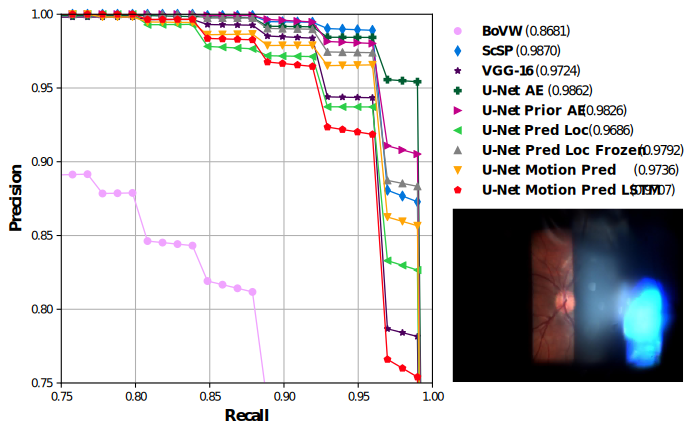
\includegraphics[width=12cm]{final_eval/ds14_pr}
  }
  \\[30pt]
  \subfloat[\textit{Max F1-Scores} of dataset \textit{Slit-Lamp Retina C}]
  {
    \label{subfig:reprod_ds14}
    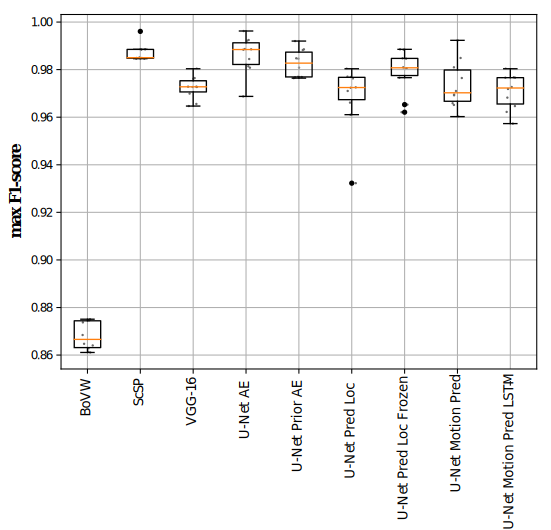
\includegraphics[width=10cm]{final_eval/ds14_reprod}
  }
  \caption[Detailed results of dataset \textit{Slit-Lamp Retina C}]{Detailed results of dataset \textit{Slit-Lamp Retina C}. (a) \textit{PR-Curves} averaged on ten repetitions. \textit{Max F1-Scores} are given in the legends. (b) Box-plot of \textit{max F1-Score} on each repetition. The median is drawn in orange.}
  \label{fig:curves_ds14}  
\end{figure}

\clearpage
\begin{figure}[!htbp]
  \centering
  \subfloat[\textit{PR-Curves} of dataset \textit{MRI Brain B} with an example image]
  {
    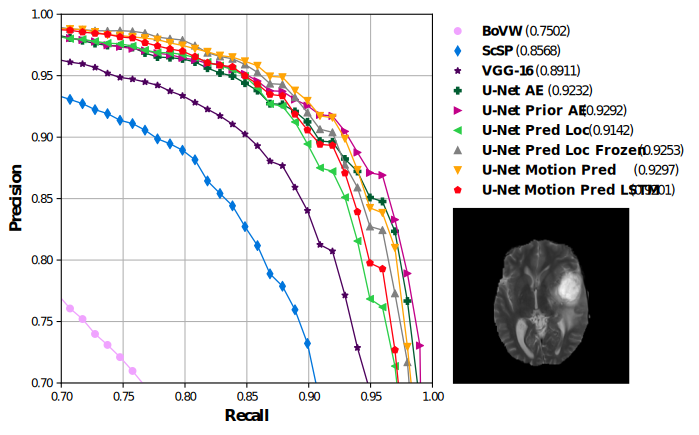
\includegraphics[width=12cm]{final_eval/ds16_pr}
  }
  \\[20pt]
  \subfloat[\textit{Max F1-Scores} of dataset \textit{MRI Brain B}]
  {
    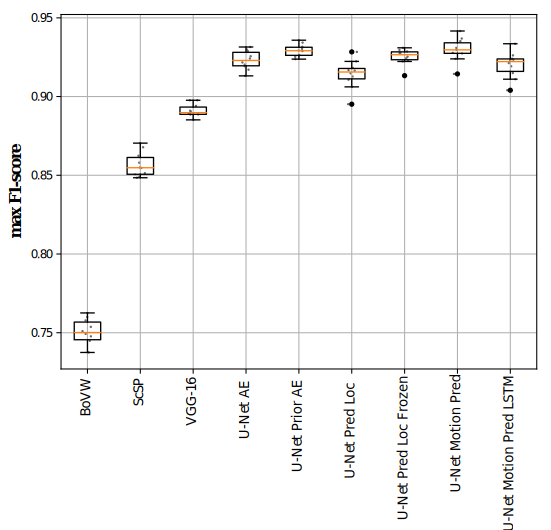
\includegraphics[width=10cm]{final_eval/ds16_reprod}
  }
  \caption[Detailed results of dataset \textit{Slit-Lamp Retina C}]{Detailed results of dataset \textit{MRI Brain B}. (a) \textit{PR-Curves} averaged on ten repetitions. \textit{Max F1-Scores} are given in the legends. (b) Box-plot of \textit{max F1-Score} on each repetition. The median is drawn in orange.}
  \label{fig:curves_ds16}  
\end{figure}

\subsection{Zero-Padding vs. Symmetric-Padding} \label{ch:zero_vs_sym_pad}
To investigate the influence of the border-effect due to zero-padding, we retrained our best model \textit{U-Net Gaze Rec} using symmetric-padding for all convolutional layers. When padding the input with symmetric property, the added pixel rows and columns are a mirror reflection of the input itself. We trained the model on one dataset per image modality. Fig. \ref{fig:activatiom_maps_sym} shows the activation maps of (a) zero-padding and (b) symmetric-padding on \textit{MRI Brain A}. The features are extracted from the last ReLU of the deepest level (see chapter \ref{ch:act_maps}).

\begin{figure}[!htbp]
  \centering
  \subfloat[Activation maps with zero-padding]
  {
    \includegraphics[height=5.8cm]{activation_maps/activations_ds09_0097_gaze_rec}
  }
  \hfill
  \subfloat[Activation maps with symmetric-padding]
  {
    \includegraphics[height=5.8cm]{activation_maps/activations_ds09_0097_gaze_rec_sympadded}
  }
  \caption[Activation maps symmetric padding]{Activation maps of a trained \textit{U-Net Gaze Rec} model with (a) zero-padding (standard configuration) and (b) symmetric-padding for the convolutional layers. The upper left image shows the passed image from \textit{MRI Brain A} datasets. The other $11$ plots show some randomly chosen activation maps, extracted at the deepest level after the last ReLU.}
  \label{fig:activatiom_maps_sym}
\end{figure}

In Tab. \ref{tab:zero_vs_sym_padd} we show the mean \textit{max F1-Scores} over ten repetitions for zero-padding (standard configuration) and symmetric-padding. There is no improvement observed.

\begin{table}[!htbp]
   \centering
   \caption[Zero vs. symmetric padding]{Comparison of zero-padding vs. symmetric-padding of the convolutional layers on a \textit{U-Net Gaze Rec} model. The values show the feature quality in terms of mean \textit{max F1-Scores} for one dataset per image modality over ten repetitions. The last column indicates the improvement due to symmetric-padding.}
   \small
   \begin{tabular}{l|c|c||c|}
      \toprule
       & \Gape[6pt][6pt]{\rotatebox[origin=cB]{90}{\parbox[t]{2.6cm}{U-Net Gaze Rec \\ \textit{\textbf{Zero-Pad}\hspace*{\fill}}}}}
       & \rotatebox[origin=cB]{90}{\parbox[t]{2.6cm}{U-Net Gaze Rec \\ \textit{\textbf{Symmetric-Pad}\hspace*{\fill}}}}
       & \rotatebox[origin=cB]{90}{\parbox[t]{2.6cm}{\textbf{Improvement\hspace*{\fill}}}} \\
      \midrule
      \textbf{Tweezer} & 0.9832 & 0.9823  & \textbf{-0.091\%} \\\midrule
      \textbf{Brain A} & 0.9810 & 0.9830 &  \textbf{+0.203\%} \\\midrule
%      {\scriptsize MRI Brain B} & \scriptsize 0.9292 & \scriptsize 0.9278 & \scriptsize -0.0014 \\\midrule
%      {\scriptsize MRI Brain C} & \scriptsize 0.9742 & \scriptsize 0.9760 & \scriptsize +0.0018 \\\midrule
%      {\scriptsize MRI Brain D} & \scriptsize 0.9463 & \scriptsize 0.9470 & \scriptsize +0.0006 \\\midrule
%      {\scriptsize MRI Brain (B-D)} & \scriptsize 0.9463 & \scriptsize 0.9431 & \scriptsize -0.0032 \\\midrule\midrule
      \textbf{Cochlea A} & 0.9621 & 0.9535 & \textbf{-0.893\%} \\\midrule
%      {\scriptsize CT Inner Ear B} & \scriptsize 0.9623 & \scriptsize 0.9566 & \scriptsize -0.0057 \\\midrule\midrule
      \textbf{Slitlamp A} & 0.9863 & 0.9860 & \textbf{-0.03\%} \\
%      {\scriptsize Slit-Lamp B} & \scriptsize 0.9747 & \scriptsize 0.9796 & \scriptsize +0.0049 \\\midrule
%      {\scriptsize Slit-Lamp C} & \scriptsize 0.9826 & \scriptsize 0.9846 & \scriptsize +0.002 \\\midrule
%      {\scriptsize Slit-Lamp D} & \scriptsize 0.9852 & \scriptsize 0.9886 & \scriptsize +0.0034 \\\midrule
%      {\scriptsize Slit-Lamp A-D} & \scriptsize 0.9785 & \scriptsize 0.9763 & \scriptsize -0.0022 \\
      \bottomrule
   \end{tabular}
   \label{tab:zero_vs_sym_padd}
\end{table}

%%% Local Variables:
%%% mode: latex
%%% TeX-master: "../../main"
%%% End:
